\documentclass[11pt]{article}

\usepackage[margin=1in]{geometry}
\usepackage[T1]{fontenc}
\usepackage{lmodern}
\usepackage{microtype}
\usepackage{amsmath, amssymb, amsthm}
\usepackage{graphicx}
\usepackage{booktabs}
\usepackage{hyperref}
\usepackage{url}
\usepackage{caption}
\usepackage{subcaption}
\usepackage{xcolor}

\hypersetup{
  colorlinks=true,
  linkcolor=blue,
  urlcolor=blue,
  citecolor=blue,
  pdftitle={Can World Models Optimize Customer Journeys and Lifetime Value?},
  pdfauthor={Benoit Bousqui\'e}
}

\newcommand{\E}{\mathbb{E}}
\newcommand{\st}{s_t}
\newcommand{\stnext}{s_{t+1}}
\newcommand{\at}{a_t}
\newcommand{\wm}{\hat{P}}
\newcommand{\gt}{P}

\title{Can World Models Optimize Customer Journeys and Lifetime Value?\\
\large A diagnostic, simulation-based framework for sequential marketing optimization}
\author{Benoit Bousqui\'e}
\date{\today}

\begin{document}
\maketitle

\begin{abstract}
World models---learned simulators of customer dynamics---offer a natural mechanism for optimizing customer journeys and customer lifetime value (CLV), where marketing actions have delayed effects through engagement, fatigue, and churn. However, learning a simulator from operational logs is challenging because action assignment is often confounded by targeting rules, and planning can amplify model error over longer horizons.
We propose a diagnostic, simulation-based framework that separates \emph{training} (learning a world model from logged trajectories) from \emph{grading} (evaluating policies in an independent ground-truth simulator), enabling direct measurement of a \emph{reality gap} between simulated and realized policy value.
In Level-0 experiments, we observe a regime-dependent reality gap: models trained on randomized logs remain comparatively conservative on the analyzed subset, while models trained on confounded logs become increasingly optimistic at longer horizons, overestimating achievable value.
\end{abstract}

\tableofcontents

\section{Introduction}
Marketing optimization has progressively moved from descriptive analytics toward prediction, causal targeting, and sequential decision-making. Customer journeys are multi-touchpoint and dynamic: interventions taken today influence future response. This motivates viewing marketing as a sequential decision problem with delayed effects and cumulative objectives such as customer lifetime value.

\paragraph{Contributions.}
\begin{itemize}
\item We present a diagnostic evaluation pipeline for journey optimization that separates world-model training from policy grading to avoid circular evaluation.
\item We propose a staged experimental program (randomized vs confounded logging, horizon and bias sweeps) that operationalizes five conceptual propositions about when world-model planning should help or fail.
\item Using a Level-0 synthetic environment with delayed fatigue/churn effects, we empirically demonstrate a regime-dependent reality gap: under confounded logs, long-horizon planning becomes over-optimistic (simulation exceeds true performance), while randomized logs are more conservative on the analyzed subset.
\end{itemize}

\section{From Response Prediction to Causal Decision Making}
Traditional response models predict outcomes such as conversion or purchase. However, targeting customers with high predicted response may not create incremental value; those customers may have converted anyway.

\subsection{Uplift modeling}
Uplift modeling estimates incremental treatment effects. For binary treatment, the individual treatment effect is:
\[
\tau_i=\E[Y^i(1)\mid X^i]-\E[Y^i(0)\mid X^i].
\]
Uplift modeling thus represents a transition from prediction (``what will happen?'') to causal prediction (``what changes because of our intervention?'').

\section{From Individual Interventions to Customer Journeys}
Uplift modeling often operates at one decision point. Customer journeys add sequential dependence: the effect of an action depends on where it occurs in the journey and on latent state:
\[
\mathrm{Effect}(\at \mid \st).
\]
The problem becomes sequential:
\[
a_t^\ast = \arg\max_{a}\E[\text{future value}\mid \st, \at=a]
\]
rather than maximizing immediate conversion.

\section{Customer Journeys as Dynamic Systems}
Customer journeys can be represented as dynamic systems. A marketer observes signals (purchases, site visits, exposures), while latent constructs (fatigue, loyalty, churn propensity) remain partially observed. This naturally motivates sequential state representation and transition modeling.

\section{A Reinforcement Learning Perspective}
An MDP formulation $M=(S,A,P,R,\gamma)$ formalizes sequential decisions. The objective:
\[
J(\pi)=\E_{\pi}\left[\sum_{t=0}^{T}\gamma^t r_t\right].
\]
Marketing interpretation: state is customer state, action is intervention, reward encodes business value (revenue, margin, churn penalty, CLV), and policy is the decision strategy.

\section{Model-Free versus Model-Based Decision-Making}
Model-free approaches learn policies/values directly. Model-based approaches learn a model of dynamics, then plan within it. World models are a modern model-based instantiation: learn $P(\stnext\mid \st,\at)$ (or latent equivalents), then plan using imagined rollouts.

\section{World Models: Concept, Adaptation, and Latent State}
A world model approximates environment dynamics sufficiently to support simulation/planning. In marketing, the true environment $P(\stnext\mid \st,\at)$ is unknown; a learned approximation $\wm(\stnext\mid \st,\at)$ is fit from logged journeys. State may be explicit (engineered features) or latent (learned representations of history).

\section{Stochasticity}
Customer behavior is stochastic; a deterministic simulator is often inadequate. A probabilistic world model can represent uncertainty as part of the decision problem rather than an error term to be minimized away.

\section{Planning with the World Model}
Given a current state $\st$, a planner evaluates action sequences over horizon $H$, simulates future states and rewards in $\wm$, and chooses the best sequence by:
\[
\hat{J}=\sum_{k=0}^{H}\gamma^k \hat{r}_{t+k}.
\]
In practice, the system executes only the next action and replans (receding horizon / MPC).

\section{Why Long-Term Value Matters}
Marketing optimization often focuses on immediate metrics; customer-level optimization may target CLV. The optimal action under short-term objectives can differ from the optimal action under long-term objectives. A world model provides a mechanism to represent delayed effects and optimize cumulative value.

\section{Relationship with Uplift Modeling}
World models are not a replacement for uplift. Uplift estimates incremental effects at a decision point; world models represent state evolution after interventions and thereby support sequential optimization. Importantly, training a world model from observational logs does not resolve identification challenges; it shifts them into learning a simulator capable of credible counterfactual journeys.

\section{The Counterfactual Problem}
Sequential marketing is counterfactual: we observe one realized trajectory but need to compare alternative action sequences. The counterfactual space grows combinatorially with horizon. World models offer a mechanism to explore this space via simulation, but do not eliminate causal requirements.

\section{The Problem of Model Error}
A planner optimizes $J(\pi\mid \wm)$, not $J(\pi\mid \gt)$. If $\wm$ is inaccurate, the resulting policy can be optimal in simulation but poor in the true environment. This risk grows with planning horizon as errors compound.

\section{The Marketing World Model as a Decision Simulator}
We summarize the closed-loop view:
\[
\text{Customer history} \rightarrow \text{State representation} \rightarrow \text{World model} \rightarrow \text{Future simulation} \rightarrow \text{Planning} \rightarrow \text{Marketing action}
\]
with feedback: action $\rightarrow$ response $\rightarrow$ new state $\rightarrow$ repeat.

\section{Related Work and Positioning}
Simulator-based RL and world models have been explored in recommender systems and user engagement optimization. Synthetic retail environments have been proposed for benchmarking. LLM-based simulated users are emerging. This work emphasizes marketing-economics objectives and focuses on when world-model answers can be trusted, using known-ground-truth staged environments.

\section{Research Questions}
We organize the empirical program around:
\begin{description}
\item[RQ1 --- Dynamics.] Can a learned world model represent customer-state transitions following interventions?
\item[RQ2 --- Optimization.] Can planning in the learned model improve cumulative value over non-sequential approaches?
\item[RQ3 --- Long-term effects.] Does explicit modeling of state transitions produce different decisions than approaches optimized for immediate response?
\item[RQ4 --- Planning horizon.] How does decision quality change as horizon increases?
\item[RQ5 --- Model uncertainty.] How do uncertainty and prediction error affect policy reliability?
\end{description}

\section{Conceptual Propositions}
\begin{description}
\item[P1.] If customer behavior has temporal dependencies, an explicit transition model should be more informative for sequential optimization than a single-step response model.
\item[P2.] The value of world-model planning should increase when actions have delayed/persistent effects.
\item[P3.] The advantage of long-horizon planning should decrease when prediction error becomes sufficiently large.
\item[P4.] Optimizing against an inaccurate world model can produce policies that perform well in simulation but poorly in the true environment (reality gap).
\item[P5.] World-model optimization should be most useful when the objective is cumulative (CLV) rather than purely immediate.
\end{description}

\section{Proposed Research Framework}
Customer history $\rightarrow$ State representation $\rightarrow$ World model $\rightarrow$ Future simulation $\rightarrow$ Planning $\rightarrow$ Marketing action, with feedback from response to state update. The core conceptual shift is from marketing prediction to marketing simulation.

\section{Proposed Experimental Program}
We specify a staged synthetic environment program with known ground-truth dynamics.

\subsection{Environment: two levels of difficulty}
\paragraph{Level 0 (primary).} Fully observable state $\st=(E_t,F_t,P_t)\in[0,1]^3$ (engagement, fatigue, propensity). Actions $A=\{\texttt{none},\texttt{email},\texttt{discount},\texttt{recommendation}\}$. Transitions follow a logistic-style update with noise and an engineered delayed cost: \texttt{discount} increases immediate purchase probability and increases future fatigue. Reward combines purchase revenue, discount cost, and churn/unsubscribe penalty when fatigue crosses a threshold.

\paragraph{Level 1 (robustness).} Partially observable: a latent segment variable modulates coefficients; marketer observes only noisy proxies. This tests latent-state modeling claims.

\subsection{Data generation}
Trajectories are logged under (a) randomized policy (unconfounded coverage) and (b) confounded rule-based ``business as usual'' policy. World models are trained separately on each.

\subsection{World model and planning}
Model complexity is staged: shallow MLP for Level 0; recurrent/latent-state model for Level 1. Planning uses rollout-based MPC with discrete actions.

\subsection{Baselines}
Random policy; single-step / myopic uplift policy; world-model planner trained on randomized logs; planner trained on confounded logs; oracle planner using true dynamics; model-free RL with unlimited simulator access (ceiling).

\subsection{Metrics and proposition mapping}
\begin{table}[t]
\centering
\caption{Metrics mapping (as specified in the draft).}
\begin{tabular}{@{}lll@{}}
\toprule
Proposition & Manipulated variable & Measured outcome \\ \midrule
P1 & Model class & Transition error vs response-model error \\
P2 & Delayed-effect strength & Sequential vs myopic value gap \\
P3 & Horizon $H$ & Policy value vs $H$ \\
P4 & Injected bias $\beta$ & Simulated value vs true value \\
P5 & Discount factor $\gamma$ & Advantage as $\gamma\rightarrow 1$ \\
\bottomrule
\end{tabular}
\end{table}

\subsection{Observed Level-0 results (this work)}
Using the implemented Level-0 environment and sweep pipeline, we directly measure Proposition P4 in the intended form: simulated policy value versus true policy value, and the resulting reality gap. We also compare randomized versus confounded logging regimes.

\paragraph{Key finding.}
Under randomized training logs (better coverage), simulated values are conservative in the analyzed subset (negative gap shrinking toward zero as $H$ increases). Under confounded logs, long-horizon planning becomes optimistic (positive gap at larger $H$), matching the failure mode described in the simulator spec: planning exploits model error and the reality gap grows with horizon under biased data.

\begin{table}[t]
\centering
\caption{Mean reality gap $\Delta = J(\pi\mid\wm) - J(\pi\mid\gt)$ for MPC policies on a matched subset ($H\in\{1,3,8,13\}$; $\gamma\in\{0.95,0.99\}$). Positive values indicate optimistic simulation.}
\label{tab:gap}
\begin{tabular}{@{}llllr@{}}
\toprule
Regime & $\gamma$ & $\beta$ & $H$ & Mean reality gap \\ \midrule
\multicolumn{5}{l}{\textbf{Randomized (subset shown, $\beta=0.0$)}}\\
Randomized & 0.95 & 0.00 & 1  & -250.00\\
Randomized & 0.95 & 0.00 & 3  & -134.49\\
Randomized & 0.95 & 0.00 & 8  &  -93.63\\
Randomized & 0.95 & 0.00 & 13 &  -39.70\\
Randomized & 0.99 & 0.00 & 1  & -250.00\\
Randomized & 0.99 & 0.00 & 3  & -148.95\\
Randomized & 0.99 & 0.00 & 8  & -104.57\\
Randomized & 0.99 & 0.00 & 13 &   10.78\\ \midrule
\multicolumn{5}{l}{\textbf{Confounded}}\\
Confounded & 0.95 & 0.00 & 1  & -108.60\\
Confounded & 0.95 & 0.00 & 3  &  -13.98\\
Confounded & 0.95 & 0.00 & 8  &   72.46\\
Confounded & 0.95 & 0.00 & 13 &  110.12\\
Confounded & 0.95 & 0.05 & 1  & -167.42\\
Confounded & 0.95 & 0.05 & 3  &  132.26\\
Confounded & 0.95 & 0.05 & 8  &   85.60\\
Confounded & 0.95 & 0.05 & 13 &  107.12\\
Confounded & 0.95 & 0.10 & 1  & -157.80\\
Confounded & 0.95 & 0.10 & 3  &   29.86\\
Confounded & 0.95 & 0.10 & 8  &   17.14\\
Confounded & 0.95 & 0.10 & 13 &   74.84\\
Confounded & 0.99 & 0.00 & 1  & -108.60\\
Confounded & 0.99 & 0.00 & 3  &   -9.00\\
Confounded & 0.99 & 0.00 & 8  &    5.58\\
Confounded & 0.99 & 0.00 & 13 &   99.34\\
Confounded & 0.99 & 0.05 & 1  & -167.42\\
Confounded & 0.99 & 0.05 & 3  &  111.54\\
Confounded & 0.99 & 0.05 & 8  &   62.58\\
Confounded & 0.99 & 0.05 & 13 &  104.90\\
Confounded & 0.99 & 0.10 & 1  & -157.80\\
Confounded & 0.99 & 0.10 & 3  &  -21.02\\
Confounded & 0.99 & 0.10 & 8  &   95.04\\
Confounded & 0.99 & 0.10 & 13 &  147.16\\
\bottomrule
\end{tabular}
\end{table}

\begin{figure}[t]
\centering
\begin{subfigure}{0.49\textwidth}
  \centering
  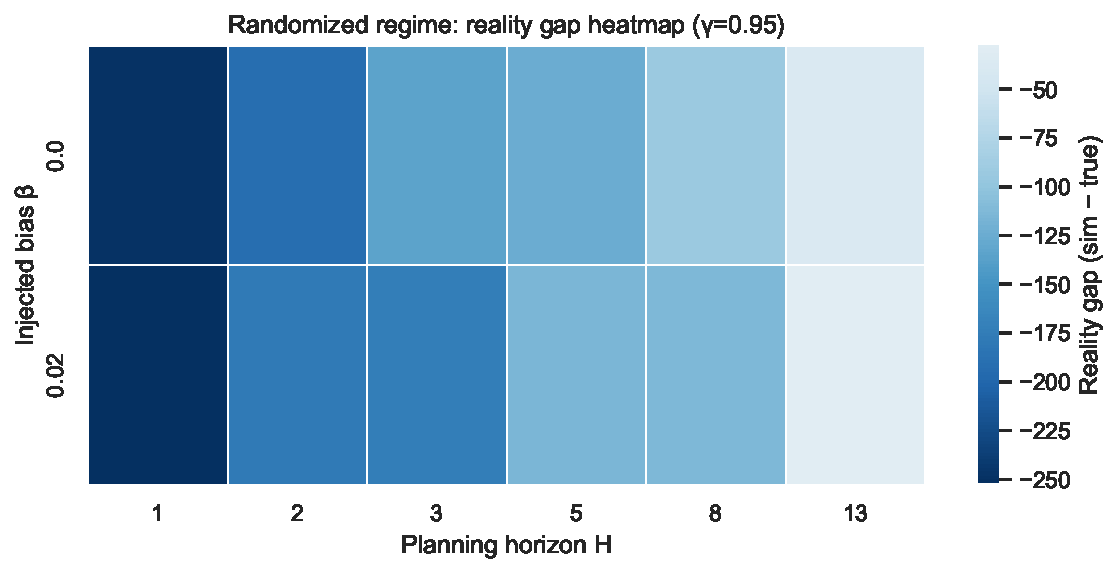
\includegraphics[width=\linewidth]{figures/fig_gap_heatmap_randomized.pdf}
  \caption{Randomized regime}
\end{subfigure}
\begin{subfigure}{0.49\textwidth}
  \centering
  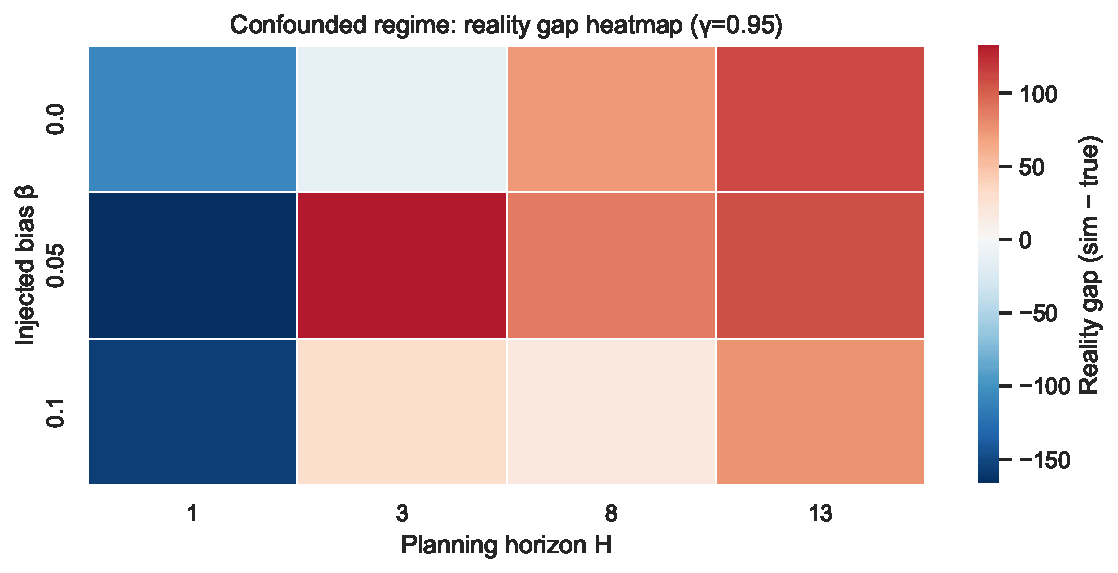
\includegraphics[width=\linewidth]{figures/fig_gap_heatmap_confounded.pdf}
  \caption{Confounded regime}
\end{subfigure}
\caption{Reality gap heatmaps (simulated minus true return) for MPC as a function of horizon $H$ and injected bias $\beta$ (figure script fixes $\gamma$).}
\label{fig:gapheatmaps}
\end{figure}

\section{Expected Contributions}
\paragraph{Conceptual.} Marketing journey optimization is framed as a world-model-based sequential decision problem positioned against adjacent recommender-systems work that optimizes engagement rather than marketing economics.

\paragraph{Methodological.} A staged, known-ground-truth environment and a causal-identification experiment (randomized vs confounded logging) are specified, with each proposition mapped to a runnable comparison.

\paragraph{Practical.} The work aims to identify conditions---in terms of planning horizon and model error---under which simulated journeys provide useful decision support, and conditions under which they do not.

\section{Limitations and Scope}
A simulated environment cannot reproduce full real-world complexity. The validity of a learned world model depends on the quality and causal informativeness of the data. External factors (competition, macro conditions) are excluded. Reward reflects a chosen objective (revenue/margin/retention/CLV). Predictive plausibility must be distinguished from causal validity. Simulation success does not imply safe deployment without additional validation and governance.

\section{Discussion}
The central conceptual shift is from marketing prediction to marketing simulation. World models add the question: ``what might happen to the customer after I act?'' This enables decision-time reasoning about consequences, but introduces a fundamental tension: longer-horizon planning increases both potential value and dependence on model accuracy. The research focus is therefore not whether a world-model marketing system can be built, but under what conditions its answers can be trusted.

\section{Conclusion}
This paper proposes learned world models as a framework for customer-journey and CLV optimization:
\[
\text{Customer state} + \text{Marketing action} \rightarrow \text{Future customer state}.
\]
Once learned, the model can simulate alternative journeys and evaluate sequences of interventions, shifting the question from ``which customer should receive this campaign?'' to ``which intervention sequence best achieves the desired long-term outcome?'' The critical empirical chain is:
\[
\text{World-model accuracy} \rightarrow \text{Simulation quality} \rightarrow \text{Planning quality} \rightarrow \text{Marketing performance}.
\]
Understanding this chain under known ground truth is essential to determine when world models represent meaningful marketing optimization versus predictive modeling with a more ambitious interface.

\bibliographystyle{plain}
\bibliography{references}

\end{document}
